% ---------- SECTION III - FOUNDATIONS ----------
% - [] Authentication and Authorisation
% - [] Password-based auth

\section{Foundations}
\label{sec:foundations}

The following chapter explains some basic concepts of web authentication and digital identities.

% ---- Authn and Authz ----
\subsection{Authentication and Authorisation}
\label{subsec:authn_authz}

Authentication and authorisation, in technical environments often referred to as \ac{authn} and \ac{authz} are concepts present in virtually every protected \ac{it} ressource.\\
The formers describes the process of identifying a user by verifying their digital identity, hence checking their \emph{authenticity}. Oftentimes only certain users are \emph{authorized} to access a protected ressource (e.g. specific parts of a website, sensitive data etc.). Therefore, an authorization has to take place both to ensure that the correct information is distributed to each user, and that no one without permission is able to manipulate data.\\
The most common and widespread type of web authentication is the so-called password-based authentication. In this case a user has to provide a \emph{username} (oftentimes an e-mail address, as these are globally unique) and a \emph{password} or \emph{passphrase}, a secret string only known to the user.\\
Only the correct combination of username and password grants access to the protected resource.

% ---- MFA ----
\subsection{Multi-Factor Authentication}
\label{subsec:mfa}

% - Often \ac{2fa} using \ac{hotp} or \ac{totp}
% - Also possible with key files
% - Only guessing or stealing the password is not enough


% ---- Federated Auth ----
\subsection{Federated Authentication}
\label{subsec:fed_auth}

% - Federated Identity Providers
% - Shibboleth, Kerberos
% - OAuth, OpenID, Login with Google/Facebook
% - Target resource (SP) never knows the password
% - User only has to remember a single password for many services, without increased risk


% ---- FIDO2 \& WebAuthn ----
\subsection{FIDO2 Overview}
\label{subsec:fido2_webauthn}

\ac{fido2} aims to provide a strong authentication factor (either as single factor for passwordless login or in a \ac{mfa} setting) using hardware keys, so called \emph{authenticators}. Those can be on the device itself (for example using \emph{Windows Hello}, Apples \emph{TouchID} or a \ac{tpm} chip), and therefore be \emph{internal} authenticators. The alternative are external or \emph{roaming} authenticators, often realised as USB keys or \ac{nfc} cards.\\
The party providing the protected ressource (e.g. a website or other web application) is referred to as \emph{relying party}.\\
The \ac{fido2} Framework consists mainly of two components: The \emph{WebAuthn} web \ac{api}, standardized by the \ac{w3c}, is the interface between the browser or \ac{os} and the authentication servers of the relying party\cite{webauthn_standard}. WebAuthn is currently supported by the Windows 10 and Android \acp{os} as well as Google Chrome, Mozilla Firefox, Microsoft Edge and Apple Safari web browsers.\cite{fido2_webauthn}\\
The second part is the \ac{ctap2} protocol that is responsible for connecting roaming authenticators to the clients device (e.g. a smartphone, laptop or personal computer).\cite{fido2_overview,fido2_ctap}\\
\\
As seen in figure \ref{fig:fido2_webauth_ctap_flow}.

\begin{figure*}[ht]
    \centering
    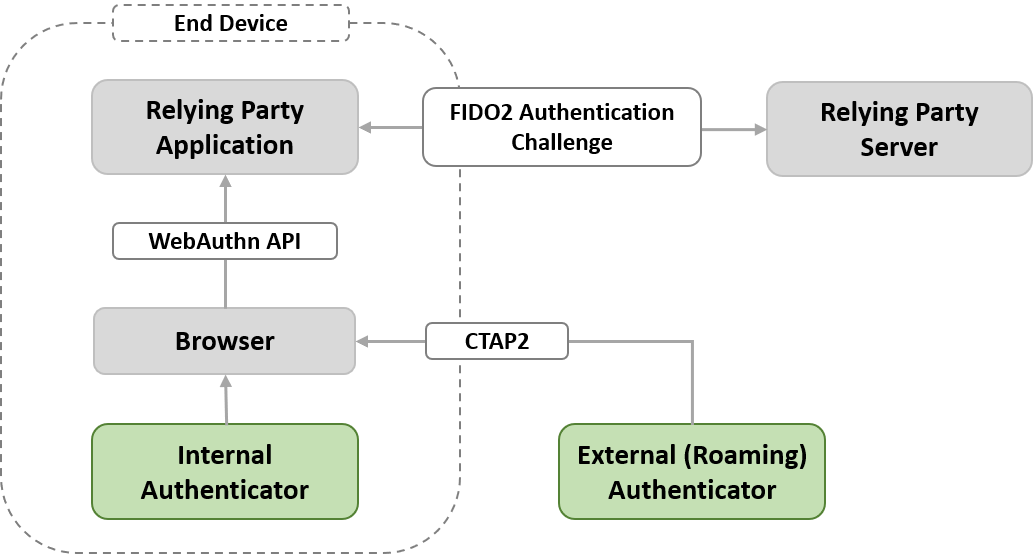
\includegraphics[width=1.8\columnwidth]{Figures/fido2_webauth_ctap_flow.png}
    \caption[FIDO2 Authentication Flow]{FIDO2 WebAuthn \& CTAP2 Authentication Flow}
    \label{fig:fido2_webauth_ctap_flow}
\end{figure*}